\section{Dimensionamento elétrico}


\begin{frame}{Introdução}
	\begin{block}{Noções iniciais}
		Nesta etapa, serão feitos os \textbf{dimensionamentos} de \textbf{todos os componentes do projeto}, calculados com base nos \textbf{dados registrados}, nas \textbf{normas técnicas }aplicáveis a cada caso e nas \textbf{tabelas de fabricantes}.

		\begin{enumerate}[a]
			\item Dimensionamento dos \textbf{condutores};
			\item Dimensionamento das \textbf{tubulações};
			\item Dimensionamento dos \textbf{dispositivos de proteção};
			\item Dimensionamento dos \textbf{quadros}.
		\end{enumerate}
	\end{block}

	\begin{block}{Observação}
		O dimensionamento dos quadros está além dos objetivos deste curso.
	\end{block}
\end{frame}


\begin{frame}{Dimensionamento dos condutores}
	\begin{block}{Seção mínima}
		\begin{itemize}
			\item A norma NBR 5410 estipula alguns critérios que devem ser levados em consideração ao se dimensionar um \textbf{condutor elétrico}.
			\item O primeiro fator a ser analisado é a \textbf{seção mínima} de cada cabo, estipulada dentro na tabela 47 da norma.
		\end{itemize}
	\end{block}
\end{frame}

%Como dimensionar cabos elétricos?
%Qual o critério mínimo para dimensionar cabos elétricos?

\begin{frame}{Dimensionamento dos condutores}
	\centering
	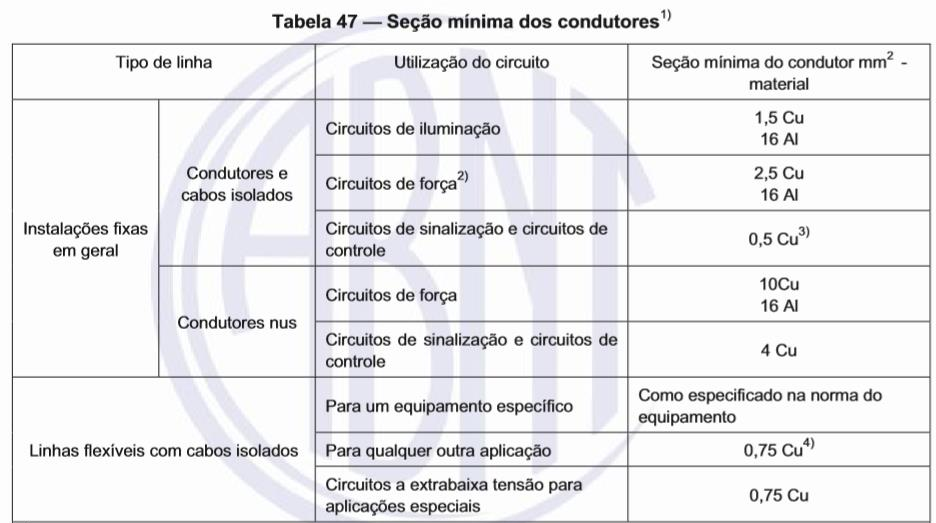
\includegraphics[width=1\linewidth]{Figuras/Ch06/fig1}
\end{frame}


\begin{frame}{Dimensionamento dos condutores}
	\begin{block}{Seção mínima}
		\begin{itemize}
			\item É importante frisar que os valores apresentados na tabela são referentes ao \textbf{critério mínimo}, ou seja, \textbf{não podem }haver cabos \textbf{menores }que esses para suas \textbf{determinadas funções}.
		\end{itemize}
	\end{block}
	\begin{block}{Método de instalação}
		\begin{itemize}
			\item Outro ponto importante é saber qual o \textbf{método de instalação do cabo}, no caso de instalações residenciais, a maior parte ocorre em \textbf{eletrodutos embutidos em alvenaria}.
			\item Segundo a tabela 33 da norma o método de instalação é o número 7 e a referência para instalação B1.
		\end{itemize}
	\end{block}
\end{frame}

%Como dimensionar cabos elétricos?
%Como escolher método de instalação dos condutores?

\begin{frame}{Dimensionamento dos condutores}
	\centering
	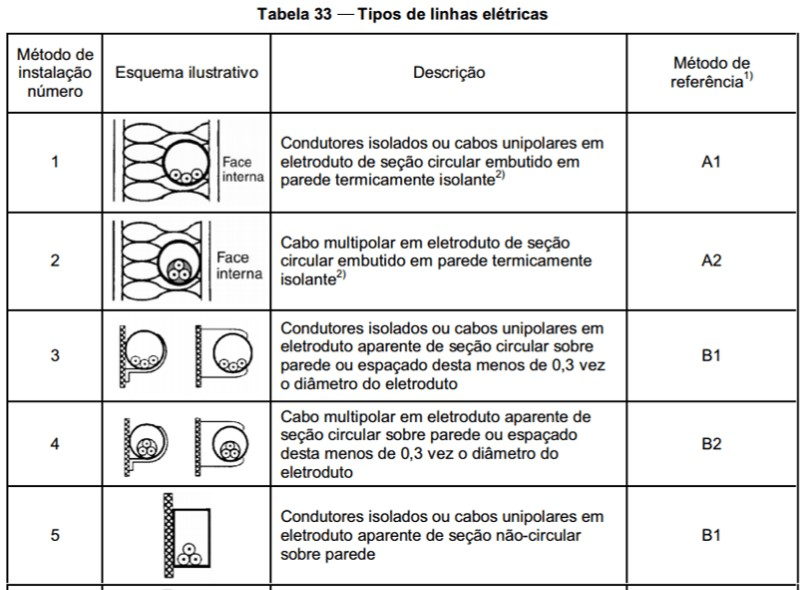
\includegraphics[width=0.85\linewidth]{Figuras/Ch06/fig2.1}
\end{frame}


\begin{frame}{Dimensionamento dos condutores}
	\centering
	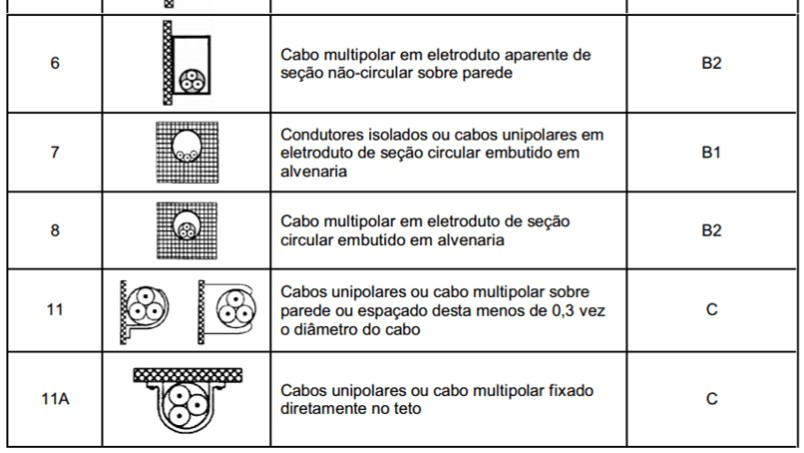
\includegraphics[width=0.9\linewidth]{Figuras/Ch06/fig2.2}
\end{frame}

\begin{frame}{Dimensionamento dos condutores}
	\begin{block}{Quantidade de cabos carregados}
		\begin{itemize}
			\item O próximo passo é descobrir qual a \textbf{quantidade ideal} de cabos carregados para o circuito.
			\item Para isso, vamos seguir as indicações da tabela 46.
			\item Observe atentamente as \textbf{especificações dos cabos}, porque esta informação será muito importante para o \textbf{dimensionamento}.
		\end{itemize}
	\end{block}
\end{frame}

%Como dimensionar cabos elétricos?
%Como determinar a quantidade de condutores carregados?

\begin{frame}{Dimensionamento dos condutores}
	\centering
	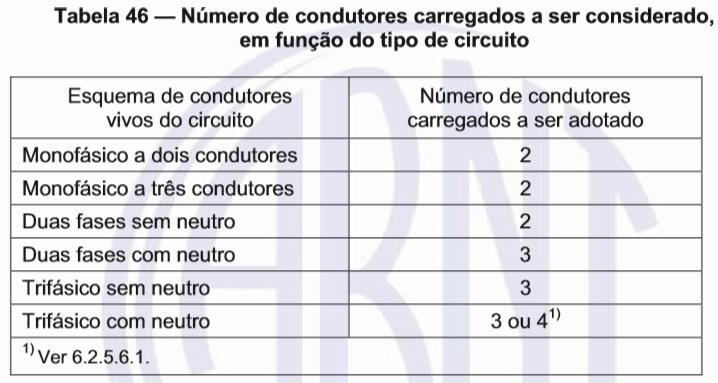
\includegraphics[width=1\linewidth]{Figuras/Ch06/fig3}
\end{frame}


\begin{frame}{Dimensionamento dos condutores}
	\begin{block}{Condução de corrente}
		\begin{itemize}
			\item Em seguida devemos consultar a tabela de \textbf{condução de corrente} - tabela 36.
			\item Esta tabela pode variar de acordo com o \textbf{tipo de condutor}, com o \textbf{tipo de isolação}, de acordo com a \textbf{temperatura do condutor} e também com a \textbf{temperatura ambiente}.
			\item Para as instalações residenciais, o cabo com \textbf{isolação em PVC} e \textbf{condutor de cobre} é o \textbf{mais utilizado}.
		\end{itemize}
	\end{block}
\end{frame}

%Como dimensionar cabos elétricos?
%Como definir a tabela de dimensionamento de cabos?

\begin{frame}{Dimensionamento dos condutores}
	\centering
	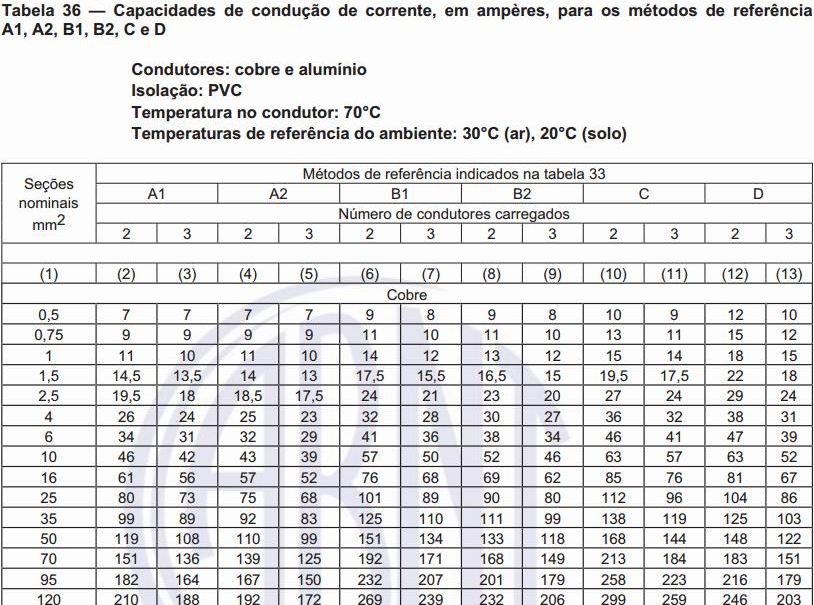
\includegraphics[width=0.85\linewidth]{Figuras/Ch06/fig4}
\end{frame}


\begin{frame}{Dimensionamento dos condutores - Exemplo \#01}
	\begin{block}{Situação}
		\begin{itemize}
			\item A corrente de projeto do circuito que será dimensionado é de \textbf{\SI{18}{\ampere}}, e o cabo utilizado tem \textbf{isolação em PVC}.
			\item O número de \textbf{circuitos dentro do eletroduto} será \textbf{4} e o \textbf{método de referência} é o \textbf{B1}, que representa o \textbf{embutido em alvenaria}.
			\item Siga a coluna do método B1, observando a quantidade de fios carregados que neste caso citado são 2, \textbf{fase e neutro}.
			\item Em seguida você deve procurar o valor de corrente mais próximo do circuito, no exemplo são \SI{18}{\ampere}.
			\item O valor \textbf{superior} mais próximo foi \SI{24}{\ampere}.
			\item Se a aplicação dos dados foi \textbf{correta}, a \textbf{tabela de dimensionamento} vai mostrar que o \textbf{cabo correto} seria o de \textbf{\SI{2.5}{\milli\meter\squared}}.
		\end{itemize}
	\end{block}
\end{frame}

%Como dimensionar cabos elétricos?
%Como definir a amperagem correta no dimensionamento de cabos?

\begin{frame}{Dimensionamento dos condutores - Exemplo \#01}
	\centering
	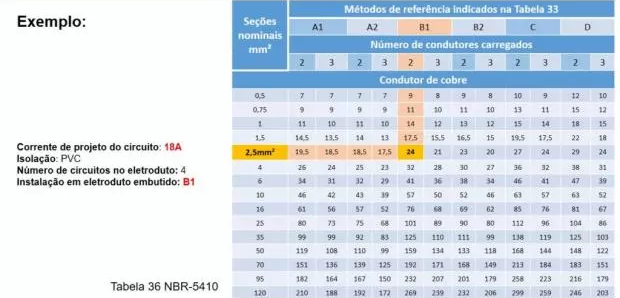
\includegraphics[width=1\linewidth]{Figuras/Ch06/fig6}
\end{frame}


\begin{frame}{Dimensionamento dos condutores}
	\begin{block}{Fator de correção}
		\begin{itemize}
			\item Mas o dimensionamento correto \textbf{não termina aqui}!
			\item É necessário levar em consideração a \textbf{quantidade de circuitos dentro do eletroduto}.
			\item Cada quantidade de circuitos requer um \textbf{fator de correção} diferente e é isso que mostra a tabela 42 da NBR 5410.
		\end{itemize}
	\end{block}
\end{frame}

%Como dimensionar cabos elétricos?
%Como calcular o fator de correção de corrente?

\begin{frame}{Dimensionamento dos condutores - Exemplo \#01}
	\centering
	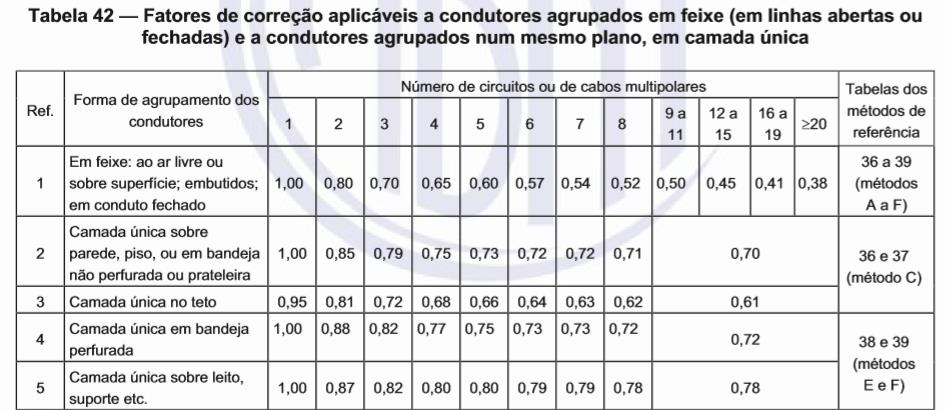
\includegraphics[width=1\linewidth]{Figuras/Ch06/fig5}
\end{frame}


\begin{frame}{Dimensionamento dos condutores - Exemplo \#01}
	\useshortskip
	\begin{block}{Capacidade de condução}
		\begin{itemize}
			\item Como o nosso exemplo utilizou \textbf{4 circuitos}, o \textbf{fator de correção} neste caso é de \textbf{\num{0,65}}.
			\item Agora você deve utilizar este fator de correção na \textbf{capacidade de condução do circuito} de \SI{2.5}{\milli\meter\squared} dentro de um eletroduto com 4 circuitos.
			\item Para isso você deve utilizar a seguinte fórmula:  \[ \boxed{I_z = I_c \cdot F_c} \]
			      onde:

			      $ I_z $ é o valor da corrente de condução do condutor corrigida, ou seja, o valor que queremos encontrar.

			      $ I_c $ é o valor da corrente de condução do condutor na tabela, ou seja, \SI{24}{\ampere}.

			      $ F_c $ é o fator de correção, ou seja, \num{0,65}.
			\item Neste caso temos $ I_z = \SI{24}{\ampere}\cdot \num{0,65}=$\textbf{\SI{15.6}{\ampere}}.
		\end{itemize}
	\end{block}
\end{frame}

%Como dimensionar cabos elétricos?
%Qual a fórmula do fator de correção de corrente?

%\begin{frame}{Dimensionamento dos condutores}
%	\centering
%	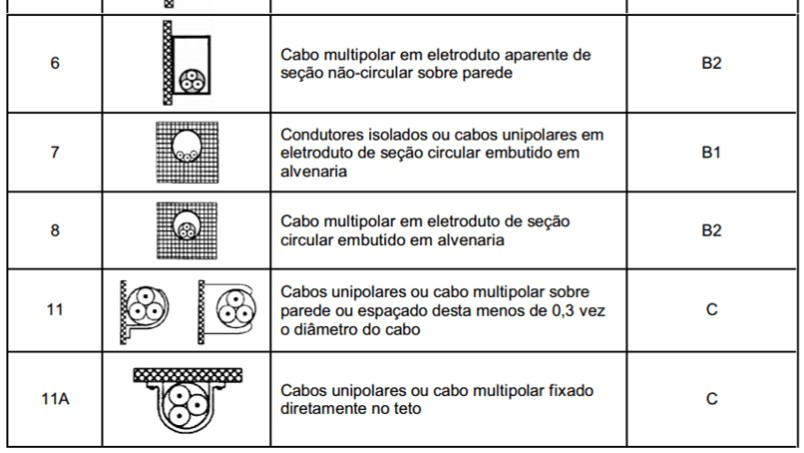
\includegraphics[width=0.9\linewidth]{Figuras/Ch06/fig2.2}
%\end{frame}


\begin{frame}{Dimensionamento dos condutores - Exemplo \#01}
	\begin{block}{Capacidade de condução}
		\begin{itemize}
			\item É importante observar se o \textbf{valor que encontrar}, no caso \SI{15,6}{\ampere} é \textbf{condizente com a condução necessária de corrente do circuito}.
			\item No exemplo utilizado a corrente é de \textbf{\SI{18}{\ampere}}, ou seja, o cabo de \SI{2,5}{\milli\meter\squared} \textbf{não vai} conseguir conduzir a corrente correta, necessitando de um cabo \textbf{mais grosso}.
			\item Voltando para a tabela de dimensionamento, o \textbf{próximo valor} dentro dos dados apresentados no exemplo é de \textbf{\SI{32}{\ampere}}.
		\end{itemize}
	\end{block}
\end{frame}

%Como dimensionar cabos elétricos?
%Qual a tabela de dimensionamento de cabo PVC?

\begin{frame}{Dimensionamento dos condutores - Exemplo \#01}
	\centering
	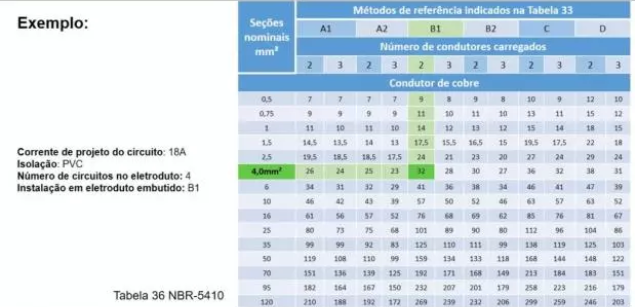
\includegraphics[width=1\linewidth]{Figuras/Ch06/fig7}
\end{frame}


\begin{frame}{Dimensionamento dos condutores - Exemplo \#01}
	\begin{block}{Conclusão}
		\begin{itemize}
			\item Jogando este novo valor na fórmula ($ I_z = I_c\cdot F_c $) do fator de correção, encontramos: $ I_z= \SI{32}{\ampere}\cdot \num{0,65}=$\textbf{\SI{20.8}{\ampere}}.
			\item Portanto, o \textbf{cabo ideal }para este exemplo apresentado é o de \textbf{\SI{4.0}{\milli\meter\squared}}.
		\end{itemize}

	\end{block}
\end{frame}


\begin{frame}{Dimensionamento dos condutores - Exemplo \#01}
	\begin{block}{Considerações finais}
		\begin{itemize}
			\item A utilização do cabo de \SI{2,5}{\milli\meter\squared} neste caso apresentado \textbf{não significa} que a instalação irá apresentar um \textbf{problema imediato}.
			\item Mas certamente haverá um \textbf{aquecimento excessivo} destes cabos, \textbf{aumentando consideravelmente o consumo de energia elétrica}.
			\item Além disso, a \textbf{longo prazo} pode haver \textbf{derretimento} da \textbf{capa isolante do cabo} acarretando em uma série de problemas.
		\end{itemize}
	\end{block}
\end{frame}


\begin{frame}{Dimensionamento das tubulações}
	\begin{block}{Noções iniciais}
		\begin{itemize}
			\item Os \textit{eletrodutos} \textbf{acomodam os cabos }pelas \textbf{paredes }de um instalação e são parte importante da \textit{infraestrutura elétrica}.
			\item Todos os componentes que \textbf{suportam}, \textbf{fixam} e \textbf{protegem cabos} e \textbf{outros componentes elétricos} fazem parte desta infraestrutura (caixas, painéis, fixadores e etc).
			\item Constituem uma parte \textbf{relativamente barata} da instalação elétrica sendo os \textbf{primeiros itens da instalação elétrica} a serem \textbf{instalados} e comumente os \textbf{primeiros da lista de compras} solicitada pelo eletricista.
			\item Talvez por serem de preço \textbf{relativamente baixo} em relação a outros componentes da instalação elétrica é que sua importância é \textbf{subestimada}.
		\end{itemize}
	\end{block}
\end{frame}


\begin{frame}{Dimensionamento das tubulações}
	\begin{block}{Normas}
		A NBR 5410 deixa bem claro que \textbf{caso seja necessária a utilização de eletrodutos}, estes devem ser \textbf{normatizados}. Existem diversas NBR’s específicas para cada tipo de eletroduto, tanto para eletrodutos embutidos quanto para eletrodutos sobrepostos. Há, basicamente, \textbf{três normas importantes} para eletrodutos:
		\begin{itemize}
			\item NBR 15465 -- Requisitos de desempenho para sistemas de eletrodutos \textbf{plásticos} para instalações elétricas de \textbf{baixa tensão}
			\item NBR 5597 -- Requisitos para eletrodutos de \textbf{aço-carbono} e \textbf{acessórios}, com \textbf{revestimento protetor} e rosca \textbf{NPT}
			\item NBR 5598 -- Requisitos para eletrodutos de \textbf{aço-carbono} e \textbf{acessórios}, com \textbf{revestimento protetor} e rosca \textbf{BSP}
		\end{itemize}
		Nas instalações elétricas residenciais o eletroduto mais comum é o \textbf{flexível corrugado}.
	\end{block}
\end{frame}


\begin{frame}{Dimensionamento das tubulações}
	\begin{block}{Disponibilidade}
		\begin{itemize}
			\item Fabricados normalmente em material \textbf{PVC} ou \textbf{similar} eles possuem um \textbf{custo baixo} e uma \textbf{boa maleabilidade} e são encontrados nas seguintes bitolas:
		\end{itemize}
	\end{block}
	\bigskip

	\centering
	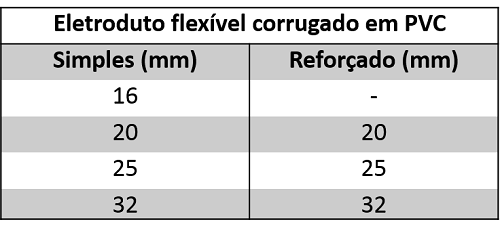
\includegraphics[width=0.7\linewidth]{Figuras/Ch06/fig8}
\end{frame}
%Tabela eletrodutos corrugados.
%Seções normatizadas para eletroduto corrugados.


\begin{frame}{Dimensionamento das tubulações}
	\begin{block}{Conversão padronizada}
		\begin{itemize}
			\item Dentro da NBR 5444 (Símbolos gráficos para instalações elétricas prediais) é estipulada uma tabela para a \textbf{conversão normatizada} de \textbf{polegadas} para \textbf{milimetro} embasada na NBR 5626 -- Instalações prediais de água fria.
		\end{itemize}
	\end{block}

	\centering
	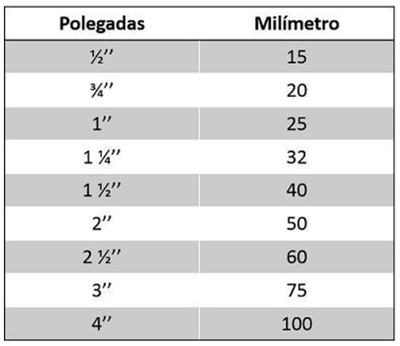
\includegraphics[width=0.45\linewidth]{Figuras/Ch06/fig9}
\end{frame}


%Tabela 1 NBR5444.
%Tabela de equivalência entre polegadas e milímetros.

\begin{frame}{Dimensionamento das tubulações}
	\begin{block}{Conversão padronizada}
		\begin{itemize}
			\item A tabela é importante pois medimos em \si{\milli\meter\squared}, porém os eletrodutos são comprados em medidas de \si{\square\pol}.
			\item Existe um método matemático que leva em consideração uma série de fatores para dimensionamento correto de um eletroduto.
			\item É importante que se tenha os \textbf{dados dos fabricantes dos condutores }para um dimensionamento correto dos eletrodutos o que é \textbf{confuso} devido a \textbf{grande quantidade de variações} na fabricação de cabos.
			\item No caso de instalações mais simples a tabela a seguir pode ser usada de modo a \textbf{referenciar} e \textbf{simplificar o dimensionamento} dos eletrodutos.
			\item Esta tabela \textbf{não é} absoluta mas sua consulta é simplificada devido a \textbf{facilidade de interpretação} e \textbf{pouca margem de erro}.
		\end{itemize}
	\end{block}
\end{frame}


\begin{frame}{Dimensionamento das tubulações}
	\centering
	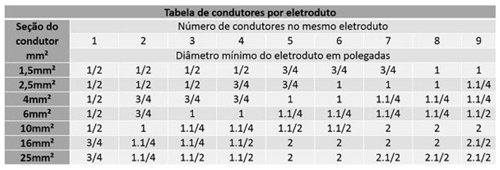
\includegraphics[width=1\linewidth]{Figuras/Ch06/fig10}
\end{frame}


\begin{frame}{Dimensionamento das tubulações}
	\begin{block}{Conversão padronizada}
		\begin{itemize}
			\item Esta tabela leva em consideração \textbf{dois critérios}: (1) a \textbf{quantidade de cabos }em um eletroduto e; (2) a \textbf{seção destes condutores}.
			\item Para sua utilização basta olhar a \textbf{coluna} contendo o \textbf{número de cabos }dentro do eletroduto em questão e, em seguida, cruzar com a \textbf{linha }referente à \textbf{seção dos cabos }dentro deste eletroduto.
			\item A casa de \textbf{interseção} entre \textbf{coluna }e \textbf{linha }resulta no \textbf{valor em polegadas }do \textbf{eletroduto adequado para comportar esses cabos}.
		\end{itemize}
	\end{block}
\end{frame}


\begin{frame}{Dimensionamento das tubulações - Exemplo \#01}
	\begin{block}{Situação}
		\begin{itemize}
			\item \textbf{Dois circuitos }de TUG's passando em um mesmo condutor.
			\item A coluna selecionada será a de \textbf{6 cabos}: dois fases, dois neutros e dois terras - um conjunto F+N+T para cada circuito.
			\item Os cabos utilizados para estes circuitos de acordo com o projeto são de \textbf{\SI{2.5}{\milli\meter\squared}}.
		\end{itemize}
	\end{block}
\end{frame}


\begin{frame}{Dimensionamento das tubulações}
	\centering
	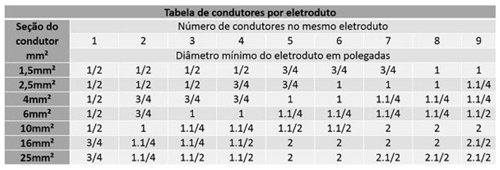
\includegraphics[width=1\linewidth]{Figuras/Ch06/fig10}
\end{frame}


\begin{frame}{Dimensionamento das tubulações - Exemplo \#01}
	\begin{block}{Resolução}
		\begin{itemize}
			\item Observando a \textbf{interseção} entre \textbf{coluna} e \textbf{linha} nota-se que o eletroduto adequado para suportar os dois circuitos do exemplo é um eletroduto de \SI{1}{\pol}.
			\item Esta tabela já leva em consideração uma \textbf{taxa adequada de ocupação} para o eletroduto, e esta taxa é importante para \textbf{garantir a temperatura adequada dentro do eletroduto} bem como a \textbf{facilidade de passagem de cabos} e \textbf{manutenção futura destes circuitos} dentro do eletroduto.
		\end{itemize}
	\end{block}
\end{frame}


\begin{frame}{Dimensionamento dos dispositivos de proteção}
	\begin{block}{Conceitos iniciais}
		\begin{itemize}
			\item O dimensionamento dos dispositivos de proteção é, de longe, o \textbf{mais complexo}.
			\item Deve-se levar em conta \textbf{tudo o que foi feito anteriormente} para que esse dimensionamento \textbf{atenda às necessidades da instalação }e \textbf{garanta a segurança de seus usuários}.
			\item Uma das \textbf{principais características} que \textbf{deve }ser atendida pelos dispositivos de proteção é a \textit{seletividade}.
		\end{itemize}
	\end{block}
\end{frame}


\begin{frame}{Dimensionamento dos dispositivos de proteção - Exemplo \#01}
	\begin{block}{Seletividade}
		\begin{itemize}
			\item \textit{Seletividade} é a propriedade que uma instalação possui de que \textbf{somente o dispositivo de proteção mais próximo do ponto de falta se desarma}.
			\item Isso garante que a parte do circuito que ficará \textbf{desligada e inoperante} seja a \textbf{menor possível}.
			\item Em nossa casa quando ocorre um curto em uma tomada, o ideal é que \textbf{apenas o circuito da tomada seja desligado }e o resto da instalação continue em funcionamento, isto é a seletividade.
			\item Para que que ocorra a seletividade é necessário que os disjuntores estejam \textbf{corretamente dimensionados}.
		\end{itemize}
	\end{block}
\end{frame}


\begin{frame}{Dimensionamento dos dispositivos de proteção - Exemplo \#01}
	\begin{block}{Situação}
		Devido à complexidade do dimensionamento dos componentes a seguir, usaremos um exemplo a fim de entender a ideia principal do processo:
		\begin{itemize}
			\item Instalação de \SI{220}{\volt}.
			\item Circuito 1 de Iluminação de \SI{900}{\watt};
			\item Circuito 2 para tomadas de TUG de \SI{1100}{\watt};
			\item Circuito 3 outro circuito de Tomadas TUG de \SI{1100}{\watt};
			\item Circuito 4 para chuveiro TUE de \SI{7500}{\watt};
			\item Circuito 5 destinado a máquina de lavar TUE de \SI{1200}{\watt};
			\item Circuito 6 para micro-ondas TUE de \SI{1100}{\watt}.
		\end{itemize}
		Os circuitos acima são separados em \textbf{iluminação}, \textbf{tomadas de uso geral} (TUG), e \textbf{circuitos especiais} que são as tomadas de \textbf{uso específico} (TUE). Eles são separados para que seja possível aplicar o \textit{fator de demanda}.
	\end{block}
\end{frame}


\begin{frame}{Dimensionamento dos dispositivos de proteção - Exemplo \#01}
	\begin{block}{Fator de demanda}
		\begin{itemize}
			\item É importante entender que os \textbf{fatores de demanda }são aplicados sobre o valor da \textbf{potência}, sendo assim, devemos aplicar o fator para \textbf{circuitos de iluminação} e \textbf{circuitos TUG}.
			\item Devemos, então, \textbf{somar as potências destes circuitos}:
		\end{itemize}
		\centerline{
			\begin{tabular}{c@{\,}c@{\,}c@{\,}c@{\,}c@{\,}l}
				  &   & 9 & 0 & \SI{0}{\watt} & potência da iluminação ativa -- circuito 1 \\
				+ & 1 & 1 & 0 & \SI{0}{\watt} & potência das tomadas TUG -- circuito 2     \\
				+ & 1 & 1 & 0 & \SI{0}{\watt} & potência das tomadas TUG -- circuito 3     \\
				\cmidrule{1-5}
				  & 3 & 1 & 0 & \SI{0}{\watt} & no total                                   \\
			\end{tabular}}
		\begin{itemize}
			\item Após obtermos o \textbf{valor total da potência} podemos consultar a tabela de \textit{fator de demanda}.
			\item Lembre-se que essas tabelas \textbf{variam de acordo com a sua região}, portanto são disponibilizadas nos \textbf{sites das concessionárias}.
		\end{itemize}
	\end{block}
\end{frame}


\begin{frame}{Dimensionamento dos dispositivos de proteção - Exemplo \#01}
	\centering
	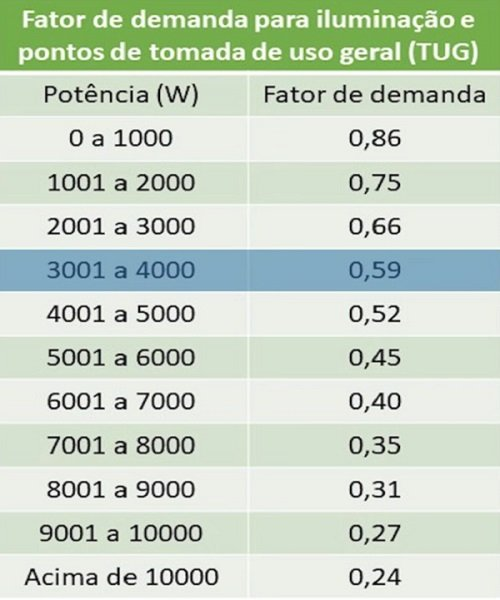
\includegraphics[width=0.5\linewidth]{Figuras/Ch06/fig12}
\end{frame}


\begin{frame}{Dimensionamento dos dispositivos de proteção - Exemplo \#01}
	\begin{block}{Fator de demanda}
		\begin{itemize}
			\item No exemplo anterior a potência total era de \SI{3100}{\watt}, ou seja, esse valor de potência na faixa de \textbf{\SI{3001}{\watt} a \SI{4000}{\watt}}, cujo \textbf{fator de demanda é \num{0,59}}.
			\item Após ter identificado, basta \textbf{multiplicar \SI{3100}{\watt} pelo fator de \num{0,59}} e obtemos a potência já ajustada que é de \textbf{\SI{1829}{\watt}}.
			\item O próximo passo é \textbf{aplicar o fator de demanda para os circuitos de uso especial} que são:

			      \centerline{
				      \begin{tabular}{c@{\,}c@{\,}c@{\,}c@{\,}c@{\,}l}
					        & 7 & 5 & 0 & \SI{0}{\watt} & chuveiro         \\
					      + & 1 & 2 & 0 & \SI{0}{\watt} & máquina de lavar \\
					      + & 1 & 1 & 0 & \SI{0}{\watt} & micro-ondas      \\
					      \cmidrule{1-5}
					        & 9 & 8 & 0 & \SI{0}{\watt} & no total         \\
				      \end{tabular}}
			\item A tabela a seguir define o fator de demanda de acordo com a quantidade dos circuitos de uso especial.
		\end{itemize}
	\end{block}
\end{frame}


\begin{frame}{Dimensionamento dos dispositivos de proteção - Exemplo \#01}
	\centering
	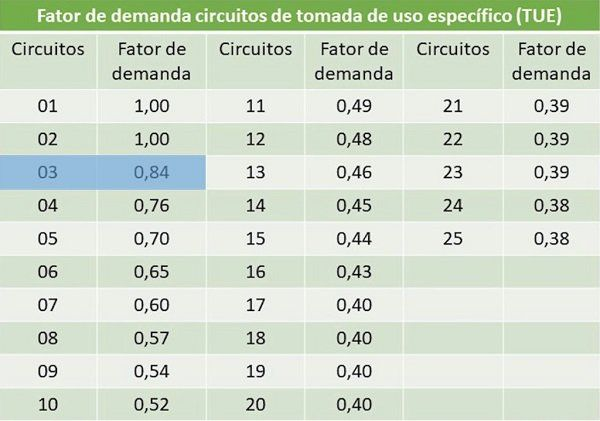
\includegraphics[width=0.8\linewidth]{Figuras/Ch06/fig11}
\end{frame}


\begin{frame}{Dimensionamento dos dispositivos de proteção - Exemplo \#01}
	\begin{block}{Fator de demanda}
		\begin{itemize}
			\item No exemplo que utilizamos, temos \textbf{três circuitos de uso especial }e, nesse caso, o fator de demanda é de \textbf{\num{0,84}}.
			\item Agora basta \textbf{multiplicarmos} a \textbf{potência de \SI{9800}{\watt}} pelo \textbf{fator \num{0,84}} para obtermos a potência (já ajustada) de \textbf{\SI{8232}{\watt}}.
		\end{itemize}
	\end{block}
	\begin{block}{Potência total}
		\begin{itemize}
			\item Após ajustarmos as potências dos circuitos, vamos achar a \textbf{potência total da instalação} ajustada \textbf{de acordo com a demanda}.
			\item Para isso basta somar a \textbf{potência de iluminação }e \textbf{tomadas TUG }mais a \textbf{potência de tomadas TUE}, totalizando \textbf{\SI{10061}{\watt}}.
		\end{itemize}
	\end{block}
\end{frame}


\begin{frame}{Dimensionamento dos dispositivos de proteção - Exemplo \#01}
	\begin{block}{Dimensionamento do disjuntor do medidor}
		\begin{itemize}
			\item Enfim, podemos dimensionar o disjuntor do medidor e, para isso, vamos consultar uma tabela simples da concessionária.
			\item Neste caso é da CEMIG, onde a b é \textbf{\SI{127}{\volt}} e  a de \textbf{linha} é \textbf{\SI{220}{\volt}}.
			\item A potência calculada está na faixa de \textbf{\num{10,1} a \SI{15}{\kilo\watt}} e, para essa instalação, o disjuntor do medidor deve ser de \textbf{\SI{60}{\ampere} e bipolar}, pois a ligação disponibilizada é de 3 fios (2F+N).
		\end{itemize}
	\end{block}
\end{frame}


\begin{frame}{Dimensionamento dos dispositivos de proteção - Exemplo \#01}
	\centering
	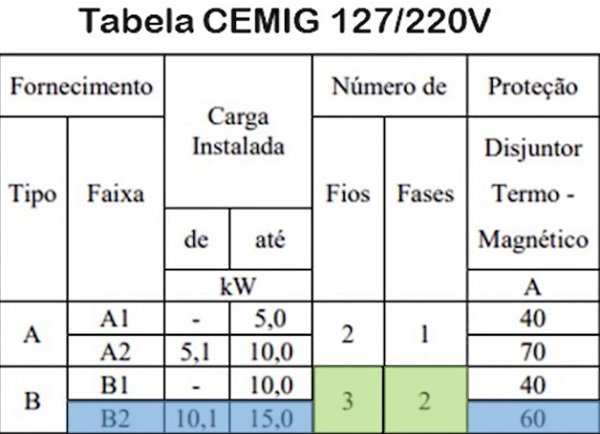
\includegraphics[width=0.8\linewidth]{Figuras/Ch06/fig13}
\end{frame}


\begin{frame}{Dimensionamento dos dispositivos de proteção - Exemplo \#01}
	\begin{block}{Dimensionamento do disjuntor do QCD}
		\begin{itemize}
			\item Para realizar o dimensionamento do disjuntor para o QDC (Quadro de Distribuição de Circuitos) vamos usar a \textbf{lei de Ohm} e dividir a \textbf{potência} pela \textbf{tensão}.
			\item Dividindo a potência de \textbf{\SI{10061}{\watt}} por \textbf{\SI{220}{\volt}}, teremos como resultado uma corrente de \textbf{\SI{45.73}{\ampere}}.
			\item Essa é a corrente para considerar no \textbf{dimensionamento do disjuntor geral do QDC}.
			\item É importante destacar que no caso da CEMIG existe a possibilidade de termos \textbf{tanto \SI{220}{\volt} quanto \SI{127}{\volt}} e, como na tabela a potência define um \textbf{disjuntor bipolar}, temos que usar a \textbf{tensão de linha} (\SI{220}{\volt}).
		\end{itemize}
	\end{block}
\end{frame}


\begin{frame}{Dimensionamento dos dispositivos de proteção - Exemplo \#01}
	\centering
	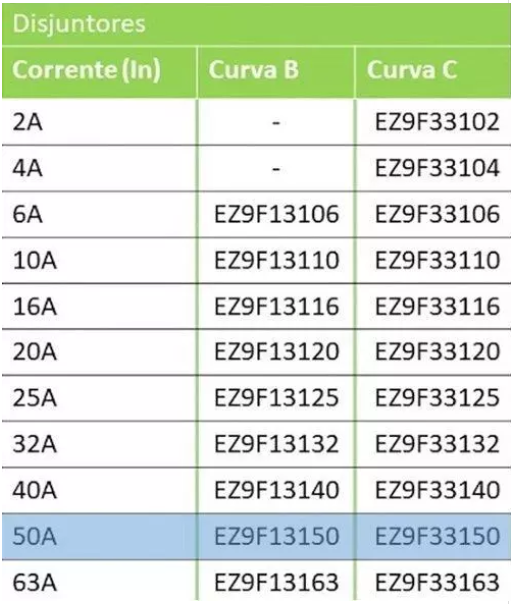
\includegraphics[width=0.5\linewidth]{Figuras/Ch06/fig14}
\end{frame}


\begin{frame}{Dimensionamento dos dispositivos de proteção - Exemplo \#01}
	\begin{block}{Dimensionamento do disjuntor do QCD}
		\begin{itemize}
			\item Após termos encontrado a corrente total do circuito, consultando uma \textbf{tabela de disjuntores}, encontramos o disjuntor de \SI{50}{\ampere} para a \textbf{corrente superior mais próxima à \SI{45,73}{\ampere}}.
			\item As curvas de disjuntores são definidas de acordo com a \textbf{utilização}, sendo o \textbf{disjuntor geral} sempre com a \textbf{maior curva} entre os disjuntores!
			\item No nosso exemplo, como há disjuntores \textbf{curvas B e C}, o disjuntor de \textbf{maior curva} deve ser usado, e \textbf{a maior curva é a C}.
			\item Podemos observar que, no caso da CEMIG, houve uma diferença entre o \textbf{disjuntor do medidor}, que é de \textbf{\SI{60}{\ampere} - bipolar}, e o \textbf{disjuntor do QDC}, de \textbf{\SI{50}{\ampere} - bipolar}.
			\item Essa diferença \textbf{não é um problema}, pois garante a \textit{seletividade} dos circuitos.
		\end{itemize}
	\end{block}
\end{frame}


\section*{Exercícios}
\frame{
	\frametitle{Exercícios}
	\begin{block}{}
		01. Explique o princípio da seletividade com suas próprias palavras.

		\bigskip

		02. Você já mexeu no disjuntor da sua casa? Faça uma estimativa de sua capacidade.
	\end{block}
}

\section*{Referências}

\frame{
	\frametitle{Referências e Exercícios Complementares}
	\begin{itemize}
		\item CREDER, Hélio; Instalações Elétricas, 14ª edição, Editora LTC, Rio de Janeiro, 2004.
		\item Manual de Instalações Elétricas - Prysmian.
	\end{itemize}
	%\centering{\alert{Página 36 - \textbf{1.6.1 até 1.6.5, 1.6.17 até 1.6.19}}} \\
	%	\centering{\alert{Lista de exercícios 01}}
}